\documentclass{article}
% translate with >> pdflatex -shell-escape <file>

% This file is an extract of the PGFPLOTS manual, copyright by Christian Feuersaenger.
% 
% Feel free to use it as long as you cite the pgfplots manual properly.
%
% See
%   http://pgfplots.sourceforge.net/pgfplots.pdf
% for the complete manual.
%
% Any required input files (for <plot table> or <plot file> or the table package) can be downloaded
% at
% http://www.ctan.org/tex-archive/graphics/pgf/contrib/pgfplots/doc/latex/
% and
% http://www.ctan.org/tex-archive/graphics/pgf/contrib/pgfplots/doc/latex/plotdata/

\usepackage{pgfplots}
\pgfplotsset{compat=newest}

\pagestyle{empty}

\begin{document}
\pgfplotsset{footnotesize,samples=10}
\begin{center}% note that \centering uses less vspace...
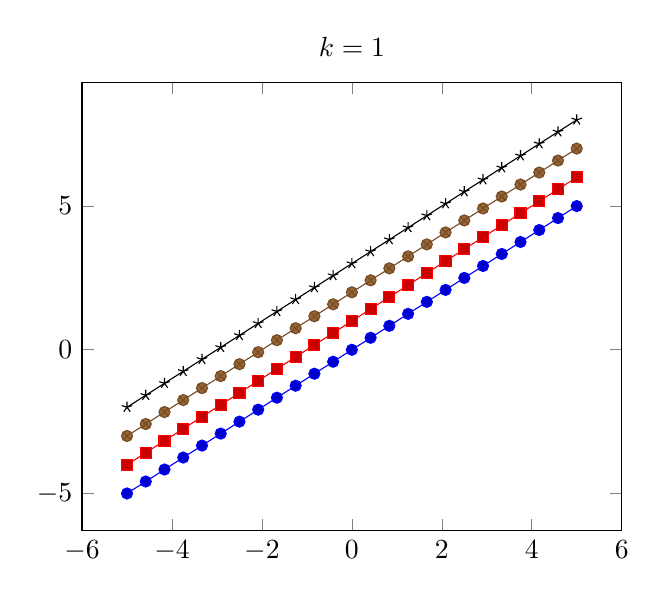
\begin{tikzpicture}
	\begin{axis}[
		legend columns=-1,
		legend entries={$(x+0)^k$;,$(x+1)^k$;,$(x+2)^k$;,$(x+3)^k$},
		legend to name=named,
		title={$k=1$}]
	\addplot {x};
	\addplot {x+1};
	\addplot {x+2};
	\addplot {x+3};
	\end{axis}
\end{tikzpicture}
%
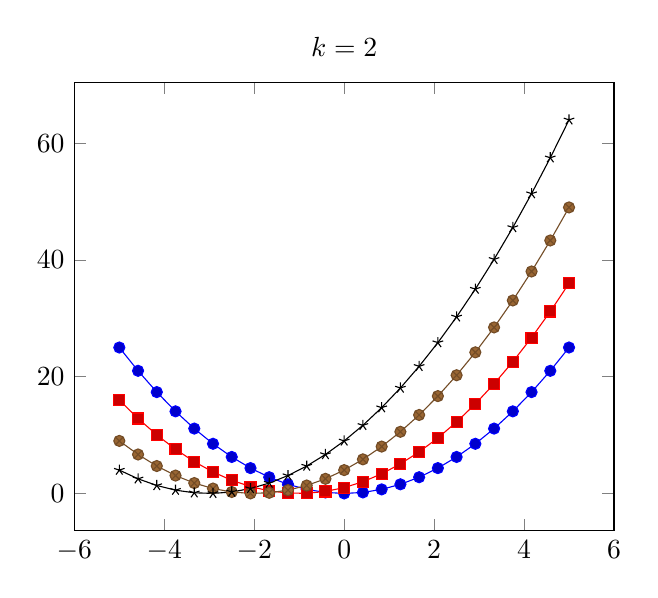
\begin{tikzpicture}
	\begin{axis}[title={$k=2$}]
	\addplot {x^2};
	\addplot {(x+1)^2};
	\addplot {(x+2)^2};
	\addplot {(x+3)^2};
	\end{axis}
\end{tikzpicture}
%
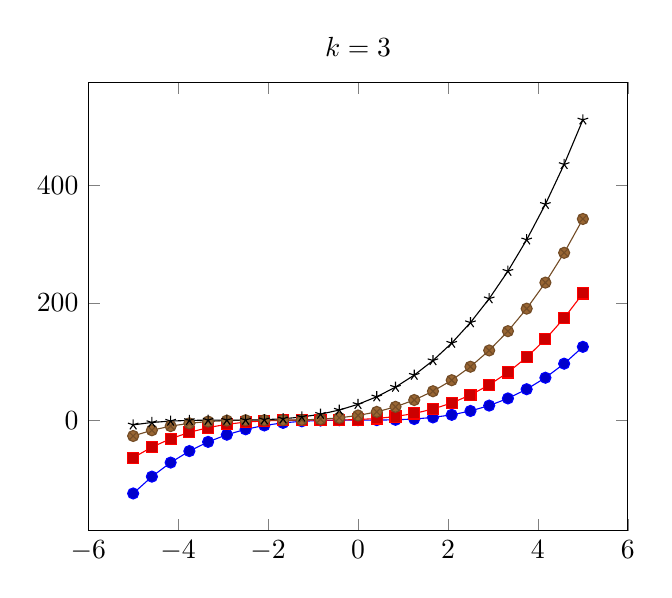
\begin{tikzpicture}
	\begin{axis}[title={$k=3$}]
	\addplot {x^3};
	\addplot {(x+1)^3};
	\addplot {(x+2)^3};
	\addplot {(x+3)^3};
	\end{axis}
\end{tikzpicture}
\\

\ref{named}
\end{center}
\end{document}
